%% \documentclass{report}
%% \usepackage{fullpage}
%% \usepackage{tikz}
%% \usepackage[utf8]{inputenc}
%% \usepackage[OT1]{fontenc}

%% \begin{document}

\begin{tikzpicture}


\node at (5,-4) {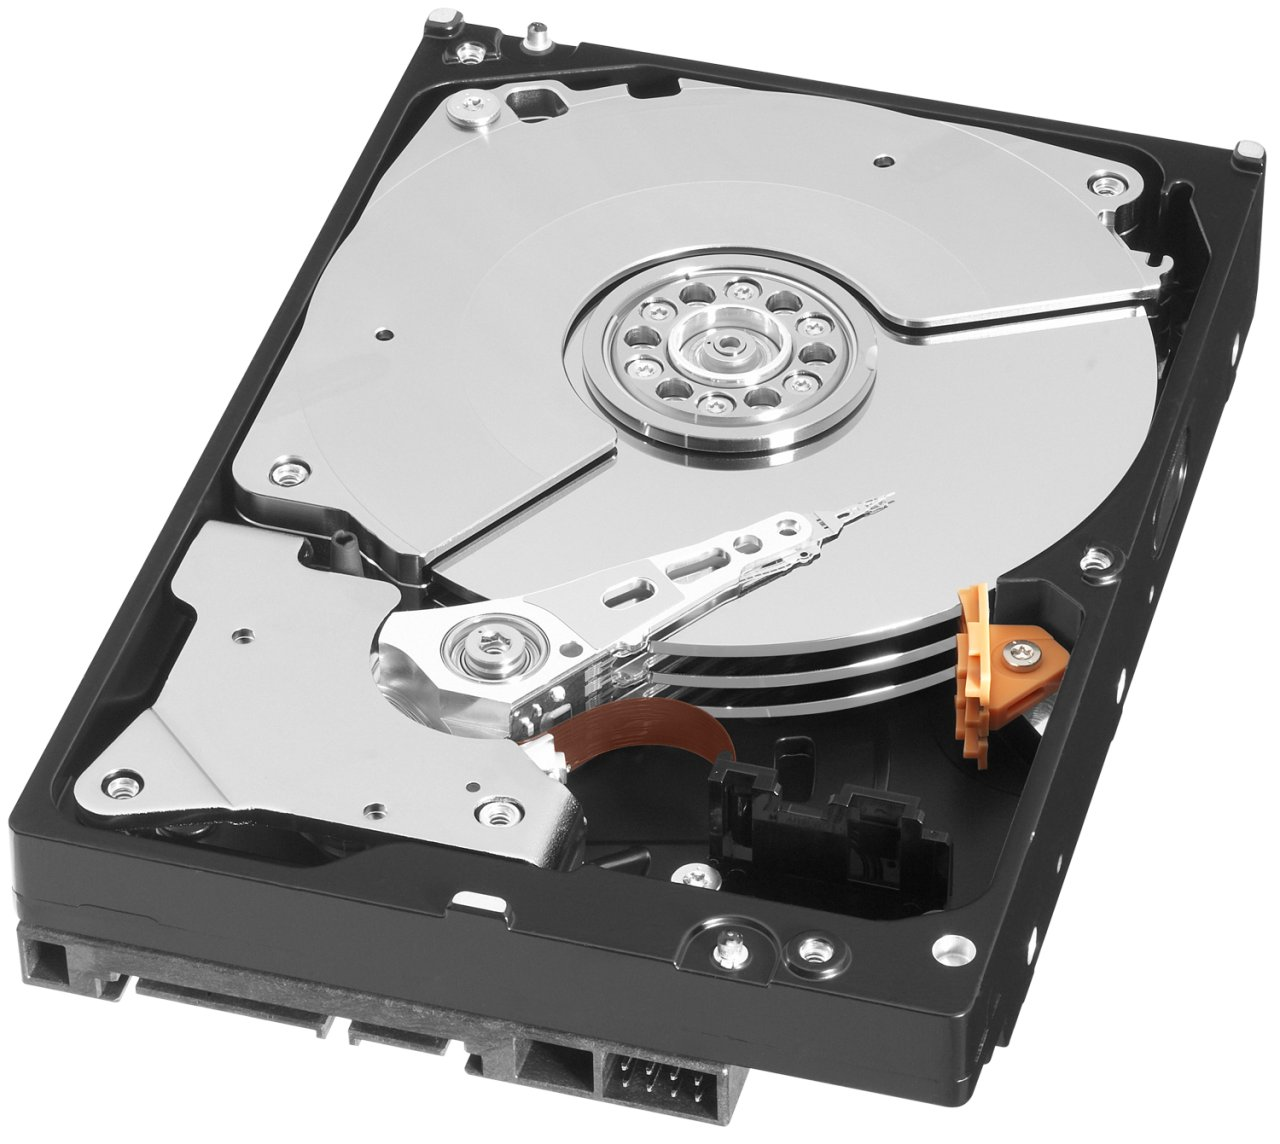
\includegraphics[width=8cm]{figures/insidedd.jpg}};


%% \foreach \i in {0,...,15} {
%%   \foreach \j in {-20,...,0} {
%%     \node[red] at (\i,\j) {\i,\j};
%%   }
%% }

\draw[blue,very thick] (7.5,-3) -- (8,-0.5) -- (9,-0.5);
\node[anchor=west] at (9,-0.5) {\Large Plateaux};

\draw[blue,very thick] (5.5,-2.6) -- (3,-0.5) -- (1.75,-0.5);
\node[anchor=east] at (1.75,-0.5) {\Large Axe de rotation};

\draw[blue,very thick] (6.5,-3.6) -- (8,-5) -- (9,-5);
\node[anchor=west] at (9,-5) {\Large Tête de lecture};

\draw[blue,very thick] (5.1,-7.2) -- (6,-8) -- (7.5,-8);
\node[anchor=west] at (7.5,-8) {\Large Alimentation};

\draw[blue,very thick] (5,-4.1) -- (3,-3) -- (1,-3);
\node[anchor=east] at (1,-3) {\Large Bras de lecture};

\draw[blue,very thick] (2.5,-6.6) -- (2,-7.5) -- (1,-7.5);
\node[anchor=east] at (1,-7.5) {\Large Interface};

\end{tikzpicture}

%\end{document}
